%$$$$$$$$$$$$$$$$$$$$$$$$$$$$$$$$$$$$$$$$$$$$$$$$$$$$$$$$$$$$$$$$$$$$$$$$$$$$$$$$
% Paragraph 3: Scalable Data Structure and Lock에 대한 연구
%$$$$$$$$$$$$$$$$$$$$$$$$$$$$$$$$$$$$$$$$$$$$$$$$$$$$$$$$$$$$$$$$$$$$$$$$$$$$$$$$
\newpage
\section{확장성 있는 락 연구}
\label{sec:lockrelated}

%$$$$$$$$$$$$$$$$$$$$$$$$$$$$$$$$$$$$$$$$$$$$$$$$$$$$$$$$$$$$$$$$$$$$$$$$$$$$$$$$
%Paragraph : 기본적인 락에 대한 이야기와 확장성 있는 락의 필요성 
%$$$$$$$$$$$$$$$$$$$$$$$$$$$$$$$$$$$$$$$$$$$$$$$$$$$$$$$$$$$$$$$$$$$$$$$$$$$$$$$$
락은 기본적으로 여러 스레드들을 안전하고 올바르게 동작하도록 만들어주는 방법이다. 
이처럼 여러 스레드를 안전하게 동작시켜주기 위해, 락은 하드웨어 동기화 명령들(CAS(Compare-And-Swap),
fetch-and-add, SWAP 등)을 이용하여 구현된다.
기본적으로 락의 구현은 코어들과 RAM간에는 공유하는 버스가 있고, 이러한 버스를 이용하여 원자적으로 처리하기 위해 
하드웨어 동기화 명령을 사용하여 구현한다. 
예를 들어 x86 시스템 같은 경우 xchg 명령어를 통해 락을 쉽게 구현할 수 있다.
하지만 실제 시스템은 보다 더 복잡한 구조를점 가지게 되는데, 
복잡한 이유는 중간에 캐시 메모리와 일관성을 유지하기 위한 
캐시 일관성 프로토콜과 매니코어 NUMA 구조에 최적화 되도록 구현해야 하기 때문이다.


%$$$$$$$$$$$$$$$$$$$$$$$$$$$$$$$$$$$$$$$$$$$$$$$$$$$$$$$$$$$$$$$$$$$$$$$$$$$$$$$$
%Paragraph : 리눅스 락 구현에 대한 이야기
%$$$$$$$$$$$$$$$$$$$$$$$$$$$$$$$$$$$$$$$$$$$$$$$$$$$$$$$$$$$$$$$$$$$$$$$$$$$$$$$$
이처럼 전통적으로 락의 primitive들은 기본적으로 두 종류로 구현되어 있는데, 
하나는 busy-waiting 방법과 다른 하나는 sleeping 락인 blocking 방법으로 구현된다.
락을 잡고 있는 시간이 적을 때는 보통 busy-waiting 방법을 사용한다. 
이 방법은 보통 락이 풀릴 때까지 전역 변수를 CAS연산을 반복적으로 수행하므로 구현된다.
이것은 blocking 방법의 문제점인 블락킹 오버헤드를 줄일 수 있으나, 수행도중 CPU를 계속 사용함에 따라 문제가 있다.
다른 방법인 sleeping 락은 락이 걸린동안 다른 스레드들을 동작시킬 수 있는 장점이 있으나, 
스케줄러의 스레드관리에 의존적이고 스케줄링 정책에 의해 락의 공정성등에 영향을 준다.


%$$$$$$$$$$$$$$$$$$$$$$$$$$$$$$$$$$$$$$$$$$$$$$$$$$$$$$$$$$$$$$$$$$$$$$$$$$$$$$$$
%Paragraph : 락과 확장성에 대한 이야기
%$$$$$$$$$$$$$$$$$$$$$$$$$$$$$$$$$$$$$$$$$$$$$$$$$$$$$$$$$$$$$$$$$$$$$$$$$$$$$$$$
최근 운영체제는 이러한 두가지 방법을 혼합하여 사용한다. 
최근 리눅스 커널의 sleeping 락은 fastpath, optimistic spinning 그리고 slowpath로 구현된 3가지의 상태의
락을 혼합하여 구현한다.
예를 들어 커널의 \code{rw\_semaphore}(reader-writer semaphore)는 아래와 같이 3가지 상태로 구현된다.
\begin{itemize}
\item \textbf{fastpath.} 아무도 락을 안잡고 있을 때, 원자적인 명령어(\code{fetch\_and\_add})를 이용하여
카운터를 수정하고 락과 함께 반환하는 부분이다.
\item \textbf{optimistic spinning.} 다른 스레드가 락을 잡고 있어서 기다려야 하는 상황이다.
하지만 optimistic spinning은 많은 부분이 락을 잡은 후 바로 반환하는 부분이 많아서 이러한 부분은 blocking 오버헤드를
줄이기 위해 busy-waiting 방법으로 수행한다. 최근에는 모든 코어가 같은 전역 변수를 읽을 경우 많은 
캐시 일관성 트래픽이 발생하므로, 락을 걸 코어에 등록하고 기다리는 코어에서는 해당 CPU의 로컬 변수만 
주기적으로 확인하는 큐기반 락(MCS 기반 락)으로 구현한다. 
\item \textbf{slowpath.} 만약 락을 잡고 있는 시간이 길어지면, 대기 큐에 집어 넣고 sleep을 수행하는 sleeping
락을 수행한다. 
\end{itemize}
이와 같이 이러한 하이브리드한 sleeping 락은 많은 성능 향상을 보인다. 

%$$$$$$$$$$$$$$$$$$$$$$$$$$$$$$$$$$$$$$$$$$$$$$$$$$$$$$$$$$$$$$$$$$$$$$$$$$$$$$$$
%Paragraph :   cache coherence 이야기
%$$$$$$$$$$$$$$$$$$$$$$$$$$$$$$$$$$$$$$$$$$$$$$$$$$$$$$$$$$$$$$$$$$$$$$$$$$$$$$$$
%캐시 일관성 때문에 발생하는 락의 오버헤드는 최근 NUMA기반의 시스템에서 큰 영향을 미치는 요소 중 하나이다.

%how does cache coherence work?
 % many schemes, here's a simple one
  %each cache line: state, address, 64 bytes of data
  %states: Modified, Shared, Invalid [MSI]
  %cores exchange messages as they read and write

%messages (much simplified)
 % invalidate(addr): delete from your cache
%  find(addr): does any core have a copy?
 % all msgs are broadcast to all cores

%how do the cores coordinate with each other?
 % I + local read -> find, S
  %I + local write -> find, inval, M
  %S + local read -> S
  %S + local write -> inval, M
  %S + recv inval -> I
  %S + recv find  -> nothing, S
  %M + recv inval -> I
  %M + recv find  -> reply, S

%can read w/o bus traffic if already S
%can write w/o bus traffic if already M
 % "write-back"

%compatibility of states between 2 cores:

 %         core1
  %        M S I
   %     M - - +
%    core2   S - + +
 %       I + + +

%invariant: for each line, at most one core in M
%invariant: for each line, either one M or many S, never both

%Q: what patterns of use benefit from this coherence scheme?
 %  read-only data (every cache can have a copy)
  % data written multiple times by one core (M gives exclusive use, cheap
   % writes)

%other plans are possible
 % e.g. writes update copies rather than invalidating
  %but "write-invalidate" seems generally the best

%Real hardware uses much more clever schemes
  %mesh of links instead of bus; unicast instead of broadcast
   % "interconnect"
  %distributed directory to track which cores cache each line
   % unicast find to directory

%$$$$$$$$$$$$$$$$$$$$$$$$$$$$$$$$$$$$$$$$$$$$$$$$$$$$$$$$$$$$$$$$$$$$$$$$$$$$$$$$
%Paragraph :   atomic instructions 이야기
%$$$$$$$$$$$$$$$$$$$$$$$$$$$$$$$$$$$$$$$$$$$$$$$$$$$$$$$$$$$$$$$$$$$$$$$$$$$$$$$$

%Q: why do we need locks if we have cache coherence?
 %  cache coherence ensures that cores read fresh data
  % locks avoid lost updates in read-modify-write cycles
   %  and prevent anyone from seeing partially updated data structures

%people build locks from h/w-supported atomic instructions
 % xv6 uses atomic exchange
  %other locks use test-and-set, atomic increment, &c
  %the __sync_... functions in the handout turn into atomic instructions

%how does the hardware implement atomic instructions?
%  get the line in M mode
%  defer coherence msgs
%  do all the steps (e.g. read old value, write new value)
%  resume processing msgs

%what is performance of locks?
 % assume N cores are waiting for the lock
  %how long does it take to hand off the lock?
   % from previous holder to next holder
  %bottleneck is usually the interconnect
   % so we'll measure cost in terms of # of msgs

%what performance could we hope for?
 % if N cores waiting,
  %get through them all in O(N) time
  %so each critical section and handoff takes O(1) time
   % i.e. does not increase with N


%$$$$$$$$$$$$$$$$$$$$$$$$$$$$$$$$$$$$$$$$$$$$$$$$$$$$$$$$$$$$$$$$$$$$$$$$$$$$$$$$
%Paragraph :   ts, ticket lock 이야기
%$$$$$$$$$$$$$$$$$$$$$$$$$$$$$$$$$$$$$$$$$$$$$$$$$$$$$$$$$$$$$$$$$$$$$$$$$$$$$$$$

%test&set spinlock (xv6/jos)
 % waiting cores repeatedly execute e.g. atomic exchange
%  Q: is that a problem?
%  yes!
%    we don't care if waiting cores waste their own time
%    we do care if waiting cores slow lock holder!
%  time for critical section and release:
%    holder must wait in line for access to bus
 %   so holder's mem ops take O(N) time
  %  so handoff time takes O(N)

%Q: is O(N) handoff time a problem?
 %  yes! we wanted O(1) time
  % O(N) per handoff means all N cores takes O(N^2) time, not O(N)


%ticket locks (linux):
 % goal: read-only spin loop, rather than repeated atomic instruction
%  goal: fairness (turns out t-s locks aren't fair)
  %idea: assign numbers, wake up one at a time
%    avoid constant t-s atomic instructions by waiters
%  Q: why is it cheaper than t-s lock?
%  Q: why is it fair?
 % time analysis:
  %  what happens in acquire?
      %atomic increment -- O(1) broadcast msg
        %just once, not repeated
      %then read-only spin, no cost until next release
    %what happens after release?
      %invalidate msg for now_serving
      %N "find" msgs for each core to read now_serving
    %so handoff has cost O(N)
    %note: it was *reading* that was costly!
  %oops, just as bad O() cost as test-and-set

%jargon: test-and-set and ticket locks are "non-scalable" locks
  %== cost of single handoff increases with N

%is the cost of non-scalable locks a serious problem?
 % after all, programs do lots of other things than locking
  %maybe locking cost is tiny compared to other stuff
  

%$$$$$$$$$$$$$$$$$$$$$$$$$$$$$$$$$$$$$$$$$$$$$$$$$$$$$$$$$$$$$$$$$$$$$$$$$$$$$$$$
%Paragraph : 락과 확장성 정리
%$$$$$$$$$$$$$$$$$$$$$$$$$$$$$$$$$$$$$$$$$$$$$$$$$$$$$$$$$$$$$$$$$$$$$$$$$$$$$$$$
이와 같이 확장성을 위해 락과 관련한 병렬 처리에서 고려해야 할 사항 정리하면 
기본적으로 락으로 보호해야 할 임계 영역(critical region)의 길이을 최대한 짧도록 해야하고, 
락 자체가 가지고 있는 오버헤드도 또한 고려해야 할 사항이다. 
또한 락의 세분화(granularity) 정도에 따라 find-grained 락을 사용할지 goarse-grained 락을 사용해야 할지 
고려해야한다.
다음으로 읽기-쓰기 비율(read-write ratios)을 고려하여 읽기가 많은 경우에는 reader-writer을 사용하고,
읽기가 많으며 stale 데이터도 괜찮은 자료구조에서는 RCU 같은 락을 사용해야 한다.  
또한 약간의 공정성(fairness) 손해보더라도 확장성을 높이는 방법도 고려해야 한다.
마지막으로 최근 락에 대해서 중요한 요소로 생각하고 있는 캐시 일관성 때문에 발생하는 
오버헤드를 고려해야 한다. 

이러한 고려사항들을 적용하여 확장성있는 락에 대한 연구는 큐 기반의
락~\cite{MellorCrummey1991MCS}~\cite{Magnusson1994QLC}, ~\cite{Wang2016BeMyGuest},
~\cite{Scott2013SS}
~\cite{Bueso2014MCS}~\cite{Bueso2015STP}과 계층적
락~\cite{Radovic2003HBL}~\cite{Chabbi2016CLL}~\cite{Luchangco2006HCQ}
~\cite{Chabbi2015HPL} 그리고 위임하는 방법(delegation
techniques)~\cite{Hendler2010FC}~\cite{Fatourou2012RCS}~\cite{Delegation2014}들이
연구되고 있다. 

\subsection{큐 기반의 락(Queued Lock)}
%\subsubsection{MCS}
%$$$$$$$$$$$$$$$$$$$$$$$$$$$$$$$$$$$$$$$$$$$$$$$$$$$$$$$$$$$$$$$$$$$$$$$$$$$$$$$$
%Paragraph :   MCS 이야기
%$$$$$$$$$$$$$$$$$$$$$$$$$$$$$$$$$$$$$$$$$$$$$$$$$$$$$$$$$$$$$$$$$$$$$$$$$$$$$$$$
모든 코어가 바라보는 전역 변수를 사용하기 때문에 발생하는 캐시 일관성 트래픽 문제는 
락 내부에서도 발생한다. 
그 동안 락의 구현은 하나의 전역변수를 대상으로 원자적 명령을 이용하여 구현하였다. 
따라서 자연히 캐시 일관성 트래픽 문제가 발생하였는데, 이것을 해결하는 방법이 큐 기반의 락을 
이용하는 것이다. 

락 때문에 발생하는 캐시 일관성 문제를 해결하기 위한 가장 쉬운 접근하는 방법은 각 
코어가 모두 다른 캐시-라인의 데이터를 가지고 스핀을 하면 쉽게 해결이 된다.
즉 각각의 코어가 read-only 스핀을 하고, 반환 하는 스레드가 명시적으로 해당 코어의 캐시-라인 데이터를 
원자적 명령을 이용하여 락을 반환하는 것이다. 
이러한 방법의 문제점은 모든 락이 모든 코어의 중복되지 않은 캐시-라인 데이터를 위한 공간을 확보해야 한다는 것이다.
이것은 현실적으로 메모리 낭비가 심히다.
이러한 문제를 해결한 것이 CLH 큐 기반 락이다. 
이러한 큐 기반의 락들의 기본 철학은 모든 코어가 같은 전역 변수를 바라 보며 스핀하지 않고, 
각자의 로컬 변수를 바라 보며 스핀하도록 하는 것이다. 
대신 락을 반환하는 스레드가 직접 해당 코어의 변수를 수정하는 일을 하는것이다. 

이러한 메모리 낭비가 심한 문제를 해결하기 위해 MCS 락이 개발되었다. 
각 락에 대한 waiter들을 링크드 리스트로 보관하자는 것이 기본적인 아이디어이고, 
이것은 하나의 스레드는 반드시 하나의 락만 기다린다는 아이디어를 활용하여 리스트로 기다리는 
스레드들을 관리하였다. 
즉 기존 많은 공간(락 * 스레드 수)이 필요할 것을 적은 공간(락 + 스레드 수)로도 구현이 가능하게 되었다.
큐 기반의 락들도 여러가지가 있으나 본 논문에서는 그 중 최근 리눅스 커널에서 사용하는 
 
%$$$$$$$$$$$$$$$$$$$$$$$$$$$$$$$$$$$$$$$$$$$$$$$$$$$$$$$$$$$$$$$$$$$$$$$$$$$$$$$$
%Paragraph 2: scalable locks의 성능에 대한 이야
%$$$$$$$$$$$$$$$$$$$$$$$$$$$$$$$$$$$$$$$$$$$$$$$$$$$$$$$$$$$$$$$$$$$$$$$$$$$$$$$$
MCS 락의 성능은 적은 코어 즉 코어 수가 2개 일경우 티켓 락이 더 좋은 성능을 보이지만, 
코어 수가 많아 질수록 MCS 락은 좋은 성능을 보인다. 
이처럼 락을 확장성 있는 락을 사용하면, 락 때문에 발생하는 확장성 문제 즉 성능이 갑자기 떨어지는 현상을 
막을 수 있으나, 근본적으로 확장성 있는 시스템을 구축하려면 반드시 임계 영역의 길이를 줄여야한다.
리눅스 커널도 역시 처음에는 티켓 락 기반의 스핀락을 사용했으나, 2013년 이후 티켓-스핀락을 MCS-스픽락으로 
변경하였다. 
엄밀하게 말하면 리눅스 커널은 MCS의 기본적인 자료구조 사이즈가 크기 때문에, 커널은 MCS 락을 커널 크기에 
맞도록 수정하여 사용한다. 
결국 2016년 부터는  리눅스 커널에서 티켓 락 기반의 스핀락은 사라지게 되었다[][].
 
%[4]. qspinlock (using MCS underneath) as the default spin-lock implementation:
 %    
      % http://git.kernel.org/cgit/linux/kernel/git/torvalds/linux.git/commit/?id=a33fda35e3a765
 
%[5]. Article providing context and motivation for various locking schemes:
 %     http://queue.acm.org/detail.cfm?id=2698990
 
%[6]. Removal of unused ticket-spinlock code from the Linux kernel:
 %    
      % http://git.kernel.org/cgit/linux/kernel/git/torvalds/linux.git/commit/?id=cfd8983f03c7b2
      

\subsection{계층적 락}

%$$$$$$$$$$$$$$$$$$$$$$$$$$$$$$$$$$$$$$$$$$$$$$$$$$$$$$$$$$$$$$$$$$$$$$$$$$$$$$$$
%Paragraph 2: 계층적 락
%$$$$$$$$$$$$$$$$$$$$$$$$$$$$$$$$$$$$$$$$$$$$$$$$$$$$$$$$$$$$$$$$$$$$$$$$$$$$$$$$
계층적인 락들은 공통적으로 스케일이 큰 NUMA 환경에서 락의 확장성을 높이는 것에 있다. 
특히 NUMA 환경에서는 원격 소켓의 데이터를 접근하는 것 때문에 성능이 저하되는 문제를,
소켓 단위로 lock의 migration을 줄여서 향상시키는 방법이다.
또한 계층적 락에 대한 연구는 여러 소켓을 global lock을 소켓 안에서 관리하는 
local lock를 두어 약간의 공정성(fairness)를 손해보더라도, 
NUMA 노드의 지역성을 향상 시켜서 성능을 향상시키는 방법이다.

\subsection{Delegation techniques}

\subsubsection{Flat Combining}

%$$$$$$$$$$$$$$$$$$$$$$$$$$$$$$$$$$$$$$$$$$$$$$$$$$$$$$$$$$$$$$$$$$$$$$$$$$$$$$$$
%Paragraph :   Flat Combining 이야기
%$$$$$$$$$$$$$$$$$$$$$$$$$$$$$$$$$$$$$$$$$$$$$$$$$$$$$$$$$$$$$$$$$$$$$$$$$$$$$$$$
Flat combining(FC)~\cite{Hendler2010FC}는 여러 코어에서 락을 각자 락을 호출하면서 명령을 수행하는 것 보다, 
하나의 코어에서 한 스레드가 해당 명령어들을 모아서 하나의 전역 락을 사용하여 처리하는 것이 보다 
효율적이고 이러한 특징을 이용한 방법이다.
그리고 이러한 철학을 하나의 알고리즘화 한 것이 FC 방법이다.
FC는 두 가지 장점을 가지는데 가장 먼저 FC는 락을 자주 수행하지 않으므로, 락에 의한 
캐시 일관성 트래픽이 상대적으로 덜 발생한다는 것이다.
다음으로 하나의 스레드에서 여러 명령어들을 수행함에 따라, 캐시 지역성이 높아져서 
여러 스레드에서 락을 걸며 수행한 방법보다 높은 성능을 가진다.

\begin{figure}[h!]
    \centering
    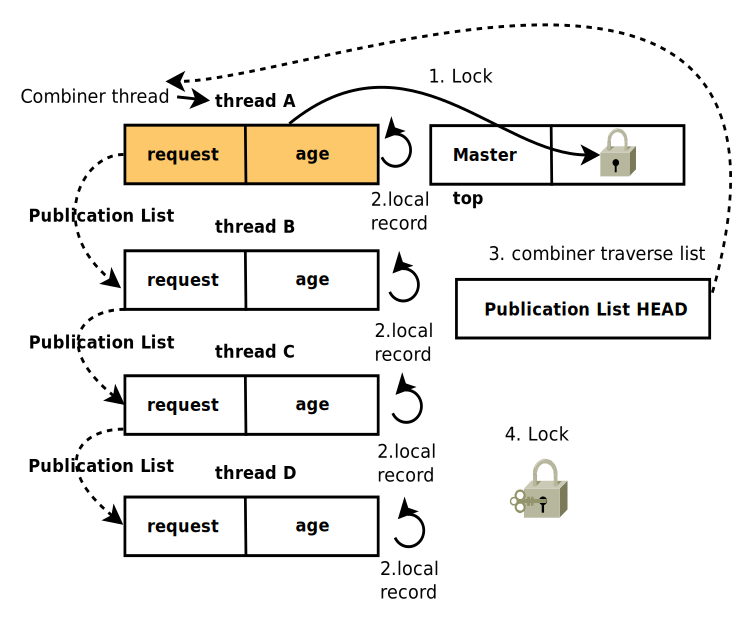
\includegraphics[width=1\textwidth]{fig/FC/FC}
    \caption{Flat combining 방법}
  \label{fig:FC}
\end{figure}

%Flat combining in shared memory.
%To access the shared stack, each thread adds its request
%to the publication list (1). Thread 4 acquires the stack’s lock and becomes the
% combiner (2), while the remaining threads spin waiting for their request to be satisfied. The combiner walks the publication list
%from the head, matching up Thread 3’s push with Thread 2’s pop on its own
% private stack (3). The two remaining pushes are added to the top of the
% shared stack (4). Finally, the top is updated, and Thread 4
%releases the lock and continues its normal executio

%$$$$$$$$$$$$$$$$$$$$$$$$$$$$$$$$$$$$$$$$$$$$$$$$$$$$$$$$$$$$$$$$$$$$$$$$$$$$$$$$
%Paragraph :   Flat Combining 알고리즘
%$$$$$$$$$$$$$$$$$$$$$$$$$$$$$$$$$$$$$$$$$$$$$$$$$$$$$$$$$$$$$$$$$$$$$$$$$$$$$$$$
그림~\ref{fig:FC}는 FC 알고리즘의 방법에 대해서 설명한다. 
먼저 자료구조에 대한 명령어(예를 들어 스택같은 경우 push 또는 pop)가 도착하면, 
처음 받은 스레드는 락을 걸고, 해당 명령어를 수행한다. 
동시에 다른 코어의 스레드들은 다른 명령어들을 수행하게 되는데, 각 코어의 스레드들은 
받은 명령어들을 코어의 내부 변수에 요청 정보과 age를 저장을 한다.
처음 받은 스레드의 명령이 끝나면 이때 부터 각 스레드에 저장된 명령을 순회하면서 combier 스레드가 
수행하고, 마지막으로 락을 푼다.

\subsubsection{OpLog}
%$$$$$$$$$$$$$$$$$$$$$$$$$$$$$$$$$$$$$$$$$$$$$$$$$$$$$$$$$$$$$$$$$$$$$$$$$$$$$$$$
%Paragraph 2: OpLog 이야기
%$$$$$$$$$$$$$$$$$$$$$$$$$$$$$$$$$$$$$$$$$$$$$$$$$$$$$$$$$$$$$$$$$$$$$$$$$$$$$$$$

\begin{figure}[h]
    \centering
    \includegraphics[width=0.8\textwidth]{fig/oplog_log}
    \caption{OpLog의 업데이트 방법}
  \label{fig:oplog}
\end{figure}


OpLog는 RCU와 반대로 업데이트 비율이 높은 업데이트 헤비(Update heavy)한 자료구조를 위해 만든 
동기화 기법 중 하나이다.
업데이트가 많아질 경우, 기존 연구들은 모두 공유 데이터를 접근함에 따라, 이때 발생하는 
캐시 일관성 트래픽이 굉장히 많이 발생한다는 것이다.
이러한 문제점을 해결하기 위한 방법 중 하나가 로그 기반으로 처리하는 것인데, OpLog는 이러한 로그 기반 
방법을 동기화된 타임스탬프 카운터를 이용하여 해결하였다. 
각 코어에 타임스탬프와 함께 명령어를 로그로 저장을 한 다음, 읽기가 수행되기 전에 
저장된 로그를 타임스탬프 정보와 함께 처리하는 방법이다.
그림~\ref{fig:oplog}는 각 코어에 저장된 로그 정보를 보여준다.
업데이트 명령어가 발생하면, 각 코어는 타임스탬프, 명령어 코드 그리고 명령어를 처리하기 위한 
정보들을 함께 저장한다.

%$$$$$$$$$$$$$$$$$$$$$$$$$$$$$$$$$$$$$$$$$$$$$$$$$$$$$$$$$$$$$$$$$$$$$$$$$$$$$$$$
%Paragraph 2: OpLog의 타임 스탬프
%$$$$$$$$$$$$$$$$$$$$$$$$$$$$$$$$$$$$$$$$$$$$$$$$$$$$$$$$$$$$$$$$$$$$$$$$$$$$$$$$
 
 
 